\section{Uncertainty Estimation}
\label{sec:uncertainty}

Data is growing bigger everyday, but that is still not enough for deep neural networks. The empirical report of \cite{mahajan2018exploring}, \cite{joulin2016learningvisual} suggests that the performance of recent deep networks is not yet saturated with respect to the size of training data, since data are mostly unlabeled. For this reason, learning methods from semi-supervised learning to unsupervised learning are attracting attention of many researchers. However, given a fixed amount of data, performance of semi-supervised or unsupervised still cannot match with that of fully-supervised learning. 
Thus, the data annotation has a vital part in uplifting the performance of neural networks
Having said that, what then is the suitable approach while the budget for annotation is limited?  \cite{atlas1989trainingconnectionist} first proposed active learning where a model actively selects data points that the model is uncertain of. The core idea of active learning is that the most informative data point would be more beneficial to model improvement than a randomly chosen data point.

Active learning has been advancing in the recent decades. Given a scenario where a labeled dataset \mathcal{L} and an unlabeled dataset \mathcal{U} is available, active learning aims to select a fixed number of subset of samples from \mathcal{U} to be labeled such that they can lead to improvement in model performance. To identify the most valuable examples to be labeled, many sampling strategies have been proposed in previous research, and it is mostly the main focus of those. Data points chosen by these strategies are expected to be able assist model to become more generalized and comprehensive after training.

Given a pool of unlabeled data, there have been two major approaches according to the selection criteria: uncertainty-based, diversity-based and expected model change

Uncertainty-based strategy [\cite{joshi2009multi}, \cite{wang2016cost}, \cite{tong2001svmactive}, \cite{seung1992query}, \cite{beluch2018power}] selects samples for which the model produces most uncertain predictions while the diversity approach [\cite{sener2018activelearningforcnn}, \cite{nguyen2004activepreclustering}, \cite{guo2010activeinstance}] selects diverse data points that can represent the entire distribution of the unlabeled pool.
Expected model change [\cite{roy2001toward}, \cite{settles2007multiple}, \cite{freytag2014selecting}] selects data points that brings great impact to the training model parameters or its outputs.

The most straightforward method of the uncertainty approach is to utilize class posterior probabilities to define uncertainty. Despite its simplicity, this approach has performed remarkably well in various tasks, such as object detection \cite{wang2018towardshuman}, semantic segmentation \cite{jain2016activesegmentationprop} and human pose estimation \cite{liu2017activehumanpose}.

Recently, Gal et al. \cite{gal2017deep} obtains uncertainty estimation from deep networks through multiple forward passes by Monte Carlo Dropout \cite{gal2016dropout}. It was shown to be effective for classification with small datasets, but according to [32], it does not scale to larger datasets.

Interestingly, \cite{yoo2019learningloss} train an additional regression module, which uses the training loss as optimization target, to predict a score for each unlabeled sample to evaluate its worthiness for labeling. 

The majority of empirical results from previous researches suggest that active learning is actually reducing the annotation cost. The problem is that most of methods require task-specific design or are not efficient in the recent deep networks.

\begin{figure}[h]
    \centering
    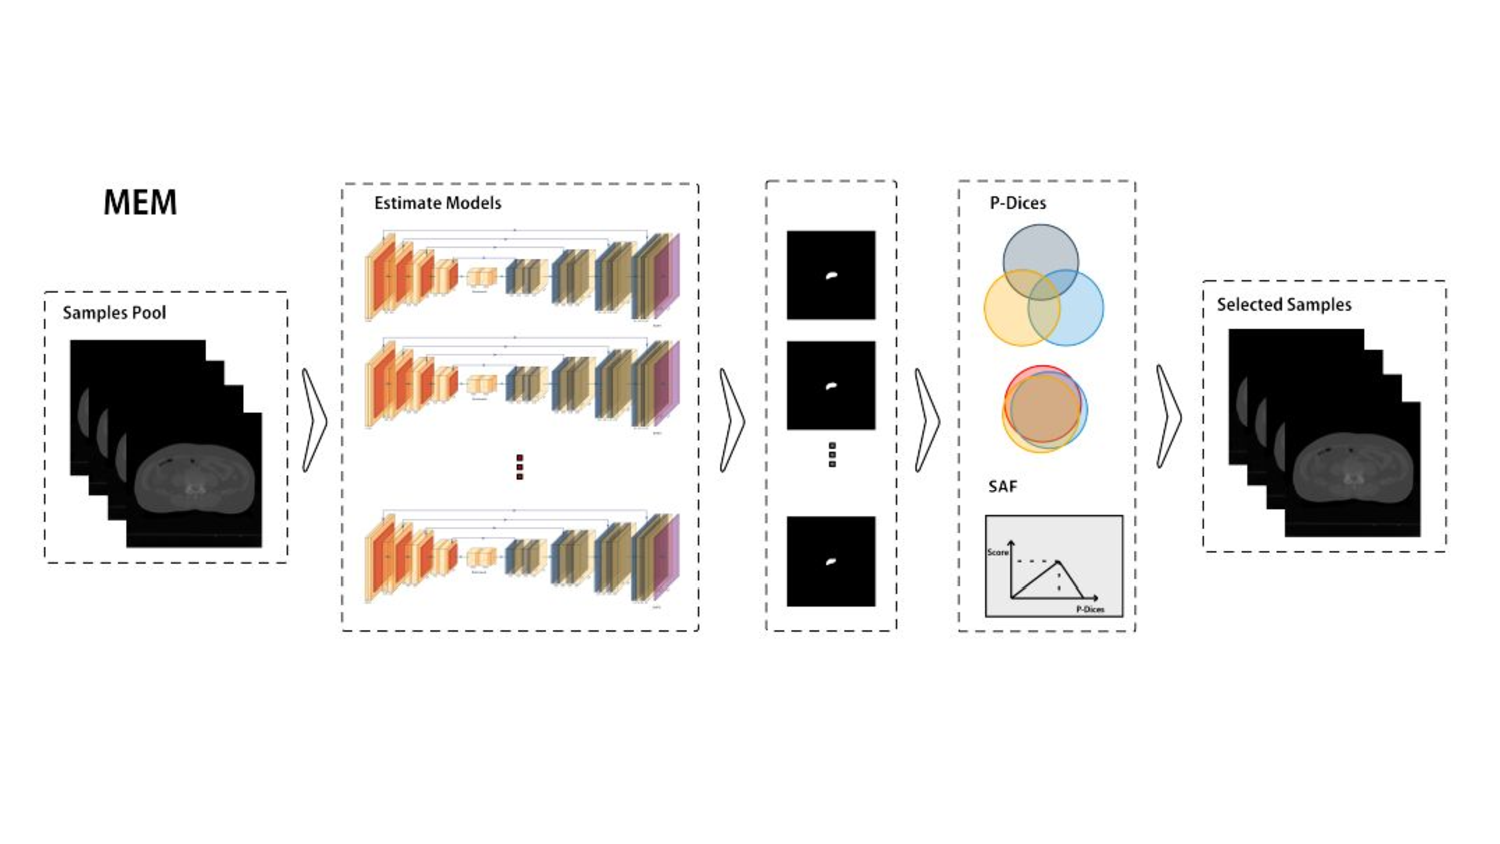
\includegraphics[width=\textwidth]{content/resources/new_images/related_works/pdices.pdf}
    \caption{A pipeline for active learning proposed in \cite{wang2019twostagequery}, which calculate unlabeled sample score through the two-step query strategy: P-Dices and SAF}
    \label{fig:pdices}
\end{figure}

As a task-agnostic uncertainty approach, \cite{seung1992query}, \cite{beluch2018power} train multiple models to construct a committee, and measure the consensus between the multiple predictions from the committee. \cite{wang2019twostagequery} goes with the same strategy where the authors compute the entropy between numerous trained agents, as depicted in Figure \ref{fig:pdices}.

We follow \cite{wang2019twostagequery} to use deep ensemble to generate prediction for each unlabeled sample, then based on consensus entropy to select good samples. While previous works aim at finding the most uncertain samples to be manually labeled by experts, but in our context, manual annotation is forbidden, therefore we try to find most certain samples that can be used for retraining.